Para graficar o plotear se puede utilizar el comando \texttt{help plot} para ver las opciones de graficado. En la Figura \ref{fig:5} se grafican distintas opciones de ploteo en Matlab.


\begin{figure}[ht!]
    \centering
    \begin{tikzpicture}
        \begin{groupplot}[group style = {
            group size = 1 by 3,
            vertical sep = 1.5cm,
        }, 
        trig format = rad,
        width=12cm, height=6cm,
        scaled y ticks = false,
        y tick label style = {/pgf/number format/fixed},
        ylabel style = {rotate = -0.45},
        title style = {font = \small}  
        ]
        \nextgroupplot[ylabel = {$x(t) = \sin t$}, title = {\texttt{plot(ax1, t, x, color = 'g', Marker = '.', MarkerSize = 10, LineStyle = 'none')}}]
        \addplot[domain = 0:10, samples = 100, green, mark = *, only marks]{sin(x)};

        \nextgroupplot[ylabel = {$x(t) = \sin t$},title = {\texttt{plot(ax2, t, x, color = 'black', Marker = 'diamond', MarkerSize = 10, LineStyle = 'none')}}]
        \addplot[domain = 0:10, samples = 100, mark = diamond, only marks, black]{sin(x)};

        \nextgroupplot[xlabel = {$t[s]$}, ylabel = {$x(t) = \sin t$}, title = {\texttt{plot(ax3, t, x, color = 'magenta', Marker = '\^ ', MarkerSize = 10, LineStyle = '-.')}}]
        \addplot[domain = 0:10, samples = 100, magenta, mark = triangle*, mark size = 3pt, dotted, mark repeat = 2,line width = 1pt, mark options = {solid, trig format = deg}]{sin(x)};
        \end{groupplot}
    \end{tikzpicture}
    \caption{Personalización de gráficos en Matlab}
    \label{fig:5}
\end{figure}

\newpage

Analicemos la siguiente función de transferencia:

\begin{equation}
    G(s) = \frac{1}{s^2 + 4s + 3}
\end{equation}

\noindent Si sometemos al sistema a una entrada impulso entonces su respuesta es según la Figura \ref{fig:6}. 

En el Código \ref{cod2} se muestra el código corregido

\begin{figure}[ht!]
    \centering
    \begin{tikzpicture}
        \begin{axis}[
            scaled y ticks = false,
            y tick label style = {/pgf/number format/fixed},
            xlabel = {$t[s]$},
            ylabel = {$y$},
            grid = both,
        ]
            \addplot[red, very thick]table[x = t, y = y]{impulso_response.txt};
        \end{axis}
    \end{tikzpicture}
    \caption{Respuesta del sistema ante la entrada impulso durante 15 segundos.}
    \label{fig:6}
\end{figure}


\begin{figure}[ht!]
    \begin{lstlisting}[caption = {Código corregido según la Guía 06.}, label = {cod2}]
    % 1. Variables: falta definir d y e
    a=1; b=100; c=1; d = 1; e = 10;

    % 2. Sumar los parametros:
    suma1 = sum([a b c d e]);


    % 3. Crear una variable s para G(s): falta encerrar entre comillas a s
    s = tf('s');

    % 4. Funcion de transferencia: falta multiplicar. Ademas tengo que borrar
    % la variable 'sum' del workspace para que funcione correctamente 

    Fs = (a*s+b)/(c*s^2+d*s+e);

    % 5. Sumar los parametros de nuevo: anteriormente declare una variable sum
    % y sum es una funcion reservada de Matlab. Hay que cambiar el nombre de la
    % variable de arriba

    suma_2 = sum([a b c d e]); 

    % 6. Respuesta ante un escalon: aca hay que cambiar el orden [y, t]
    [y, t] = step(s/(s^2+s));

    % 7. Definir los vectores "t" y "x": se cambia el 0.5 por 0.1 para el paso
    tx = 0 : 0.1 : 12;
    x = sin(0 : 0.1 : 12);

    % 8. Graficar "x" sobre "t":
    plot(tx,x) 
    \end{lstlisting}
\end{figure}


\clearpage % Vacía flotantes pendientes e inicia una página nueva limpia
\noindent % Evita la sangría inicial del párrafo
\begin{minipage}{\textwidth}
    \centering
    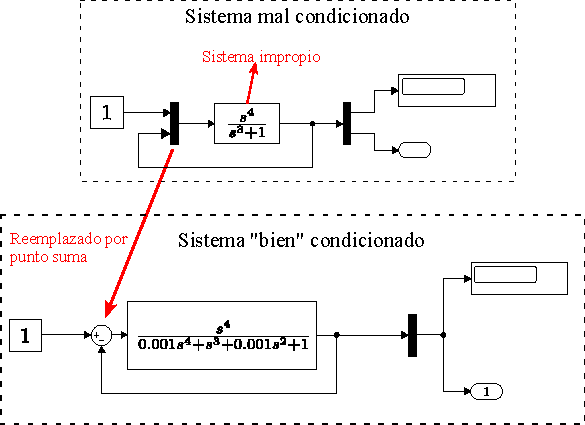
\includegraphics[width=0.8\textwidth]{imagenes/sistema_mal_condicionado.pdf}
    \captionof{figure}{Sistema hecho en Simulink. Se observa que en el sistema mal acondicinado la función de transferencia es impropia (no puede transformar el sistema en el espacio de estados), por lo tanto su solución es agregar un poco de ``ruido"\ en el denominador y de esa forma coincida con el grado del numerador. El otro error es el Mux. Para que el sistema sea retroalimetando es necesario que exista un punto suma entre la entrada y la salida del sistema para calcular el error asociado.}
    \label{fig:imagen_top}
\end{minipage}



